\documentclass[preprint]{elsarticle}
\usepackage[margin=1in]{geometry}
\usepackage{hyperref}
\usepackage{amsmath}
\usepackage{mathrsfs}
\usepackage{float}
\graphicspath{{figures/}}
%\setlength\parindent{0pt}


\makeatletter
\def\ps@pprintTitle{%
 \let\@oddhead\@empty
 \let\@evenhead\@empty
 \def\@oddfoot{\centerline{\thepage}}%
 \let\@evenfoot\@oddfoot}
\makeatother

%\usepackage{lineno,hyperref}
%\modulolinenumbers[5]

%\journal{Journal of \LaTeX\ Templates}

%%%%%%%%%%%%%%%%%%%%%%%
%% Elsevier bibliography styles
%%%%%%%%%%%%%%%%%%%%%%%
%% To change the style, put a % in front of the second line of the current style and
%% remove the % from the second line of the style you would like to use.
%%%%%%%%%%%%%%%%%%%%%%%

%% Numbered
%\bibliographystyle{model1-num-names}

%% Numbered without titles
%\bibliographystyle{model1a-num-names}

%% Harvard
%\bibliographystyle{model2-names.bst}\biboptions{authoryear}

%% Vancouver numbered
%\usepackage{numcompress}\bibliographystyle{model3-num-names}

%% Vancouver name/year
%\usepackage{numcompress}\bibliographystyle{model4-names}\biboptions{authoryear}

%% APA style
%\bibliographystyle{model5-names}\biboptions{authoryear}

%% AMA style
%\usepackage{numcompress}\bibliographystyle{model6-num-names}

%% `Elsevier LaTeX' style
\bibliographystyle{elsarticle-num}
%%%%%%%%%%%%%%%%%%%%%%%

\begin{document}

\begin{frontmatter}

\title{Title here}

%% Group authors per affiliation:
\author[add]{Authors}
\address[add]{address}
%\author{Elsevier\fnref{myfootnote}}
%\address{Radarweg 29, Amsterdam}
%\fntext[myfootnote]{Since 1880.}
%
%%% or include affiliations in footnotes:
%\author[mymainaddress,mysecondaryaddress]{Elsevier Inc}
%\ead[url]{www.elsevier.com}
%
%\author[mysecondaryaddress]{Global Customer Service\corref{mycorrespondingauthor}}
%\cortext[mycorrespondingauthor]{Corresponding author}
%\ead{support@elsevier.com}
%
%\address[mymainaddress]{1600 John F Kennedy Boulevard, Philadelphia}
%\address[mysecondaryaddress]{360 Park Avenue South, New York}

\begin{abstract}

\end{abstract}

\begin{keyword}

\end{keyword}

\end{frontmatter}

%\linenumbers

\section{Introduction}

%\begin{itemize}
%\item motivation (prediction, inference, control)
%\item background (short lit review: LWR $\rightarrow$ ARZ progression, why second order models)
%\item First order models. Defined by mass conservation and fundamental diagram. Shortcomings. No spontaneous momentum. Need to setup entropy condition. Practically used: prediction, inference. Discretized or semi-analytic solution.
%\cite{LW}
%\cite{Richards}
%\item Second order models. 
%\item goals of paper
%\item organization of paper
%\end{itemize}


Around the world traffic congestion causes a drain on the economy due to time and fuel wasted and collisions associated with traffic congestion. In 2011 congestion in America alone caused a loss of \$121 billion due to 5.5 billion hours of extra travel time and 2.9 billion gallons of wasted fuel. Although congestion levels in America are much higher now than several decades ago, they have dropped below the peak in 2005, but will increase when the economy improves \cite{Texas}. As personal vehicle ownership increases globally, traffic congestion continues to be a persistent problem. It is no surprise then that research in the physics of traffic developed with the ultimate goal of mitigating road traffic.

Traffic control strategies such as ramp metering and variable speed limits are in place today, but a good model of traffic dynamics is needed for proper coordination of control strategies. The 1950’s saw the development of the Lighthill-Whitham-Richards (LWR) model \cite{LW} \cite{Richards}, which became the seminal model for traffic flow, still studied today. This model is a conservation law for vehicles, based on fluid dynamics. Yet as a first-order model it has inherent shortcomings, such as non-physical predictions of vehicle speed as a vehicle passes through a shock and the inability to describe jamitons, phantom traffic jams which seem to appear for no reason. This prompted the development of second-order models, the prototype of which is the Payne-Whitham (PW) model \cite{payne1971models} \cite{whitham1974linear}. This and later second-order models consist of two equations, the first being the LWR equation and the second a momentum equation analogous to that describing fluid flow. Daganzo later published a study of the serious flaws of second-order traffic models, namely the emergence of gas-like behavior. While the second-order models up to that point were able to capture physics that the LWR model could not, these “improved” models also lost the anisotropy of the LWR model, incorrectly predicting that vehicles are affected by vehicles from behind \cite{Dag_requiem}. Soon after, Aw and Rascle, and independently Zhang, developed the ARZ model which avoided the inconsistencies of earlier higher-order models \cite{AR} \cite{Z}. 




\section{The ARZ model}

%\begin{itemize}
%\item physical description of ARZ model + usual form
%\item $(v, q)$ form, well-posedness 
%\end{itemize}

Aw and Rascle \cite{AR} and Zhang \cite{Z} independently developed a macroscopic second-order model of traffic flow to address the shortcomings of previously existing higher-order models. The (AR) model proposed by Aw and Rascle consists of the usual vehicle conservation and momentum equations:
\begin{align} 
\rho_t + (\rho v)_x &= 0, \label{AR1} \\
(v + p(\rho))_t + v(v + p(\rho))_x &=0 \label{AR2},
\end{align}
where $v(x,t)$ and $\rho(x,t)$ are the density and velocity, respectively, and $p(\rho)$ is a smooth, increasing function analogous to the pressure term in fluid flow. Aw and Rascle demonstrate in \cite{AR} that ``with a suitable choice of function $p$," the above class of models avoids inconsistencies of earlier second-order models. 
Zhang proposed in \cite{Z} the same model with $p(\rho) = -V(\rho)$, where $V(\rho) = Q(\rho)/\rho$ is the equilibrium velocity profile, and $Q(\rho)$ is the density-flow relation given by the fundamental diagram. In this paper we consider the Aw-Rascle-Zhang (ARZ) model with a relaxation term:
\begin{align} 
\rho_t + (\rho v)_x &= 0, \label{ARZ1} \\
(v + p(\rho))_t + v(v + p(\rho))_x &=\dfrac{V(\rho) - v}{\tau} \label{ARZ2},
\end{align}
where $\tau$ is the relaxation time. Without the relaxation term cars never reach the maximum allowable speed \cite{R_improved}. Note that at the equilibrium velocity this term is zero. 

In vector form the ARZ model is
\begin{equation} \label{ARZrhov}
\begin{pmatrix}
\rho \\ v
\end{pmatrix}_t
+ \begin{pmatrix}
v & \rho \\
0 & v + \rho V' (\rho)
\end{pmatrix}
\begin{pmatrix}
\rho \\ v
\end{pmatrix}_x = 
\begin{pmatrix}
0 \\ \dfrac{V(\rho) - v}{\tau}
\end{pmatrix}.
\end{equation}

With the appropriate variable change, we can rewrite the model in the denisty-flow and velocity-flow forms, the latter of which is most useful to us for practical control purposes. Using the flow relation $q = \rho v$ and \eqref{ARZrhov}, the density-flow form is
\begin{equation} \label{ARZrhoq}
\begin{pmatrix}
\rho \\ q
\end{pmatrix}_t
+ \begin{pmatrix}
0 & 1 \\
-\frac{q}{\rho} \left(\frac{q}{\rho} + \rho V'(\rho) \right) & 2\frac{q}{\rho} + \rho V'(\rho) 
\end{pmatrix}
\begin{pmatrix}
\rho \\ q
\end{pmatrix}_x = 
\begin{pmatrix}
0 & 0 \\ 
\frac{V(\rho)}{\tau} & -\frac{1}{\tau}
\end{pmatrix} 
\begin{pmatrix}
\rho \\ q
\end{pmatrix}.
\end{equation}

In the same manner we arrive at the velocity-flow form,
\begin{equation} \label{ARZvq}
\begin{pmatrix}
v \\ q
\end{pmatrix}_t
+ \begin{pmatrix}
v + \frac{q}{v} V'\left(\frac{q}{v}\right) & 0 \\
\frac{q}{v} \left( v + \frac{q}{v} V'\left(\frac{q}{v}\right)\right) & v
\end{pmatrix}
\begin{pmatrix}
v \\ q
\end{pmatrix}_x = 
\dfrac{1}{\tau}
\begin{pmatrix}
V\left( \frac{q}{v}\right) - v \\
\frac{q}{v}V\left( \frac{q}{v}\right) - q
% \dfrac{V\left( \frac{q}{v}\right) - v}{\tau} \\ 
% \dfrac{\frac{q}{v}V\left( \frac{q}{v}\right) - q}{\tau}
\end{pmatrix}.
\end{equation}

\subsection{Linearization}
We are interested only in small deviations, $(\tilde{\rho}(x,t), \tilde{v}(x,t))$, from the equilibrium. Consider the steady flow solution $(\rho^*(x),v^*(x))(V(\rho^*) = v^*)$. Then \eqref{ARZrhov} becomes
\begin{align}
v^* \frac{d\rho^*}{dx} + \frac{dv^*}{dx}\rho^* = 0, \\
\left( v^* + \rho^* V'( \rho^*) \right)\frac{dv^*}{dx} = \dfrac{V(\rho^*) - v^*}{\tau} = 0.
\end{align}
We must have $\frac{dv^*}{dx}=0$ else $v^* + \rho^* V'( \rho^*) = 0$. Then we have also $\frac{d\rho^*}{dx} = 0$. Hence the steady-state solution is uniform along the road. 

We linearize the ARZ model \eqref{ARZrhov} about the steady-state described above. We obtain the linearized system
\begin{equation} \label{rhovlin}
\begin{pmatrix}
\tilde{\rho} \\ \tilde{v}
\end{pmatrix}_t
+ \begin{pmatrix}
v^* & \rho^* \\
0 & v^* + \rho^* V' ( \rho^*) 
\end{pmatrix}
\begin{pmatrix}
\tilde{\rho} \\ \tilde{v}
\end{pmatrix}_x = 
\begin{pmatrix}
0 & 0 \\
\dfrac{V' (\rho^*)}{\tau} & -\frac{1}{\tau}
\end{pmatrix}
\begin{pmatrix}
\tilde{\rho} \\ \tilde{v}
\end{pmatrix}
\end{equation}

Similarly for the density-flow system \eqref{ARZrhoq}, we linearize about the equilibrium $(\rho^*, q^*)(\rho^*V(\rho^*) = q^*)$ with deviations $(\tilde{\rho}(x,t), \tilde{q}(x,t))$. The linearized system is as follows 
\begin{equation} \label{rhoqlin}
\begin{pmatrix}
\tilde{\rho} \\ \tilde{q}
\end{pmatrix}_t
+ \begin{pmatrix}
0 & 1 \\
\alpha^* \beta^* & \alpha^* - \beta^* 
\end{pmatrix}
\begin{pmatrix}
\tilde{\rho} \\ \tilde{q}
\end{pmatrix}_x = 
\begin{pmatrix}
0 & 0 \\
\delta & \sigma
\end{pmatrix}
\begin{pmatrix}
\tilde{\rho} \\ \tilde{q}
\end{pmatrix},
\end{equation}
where $\alpha^* = \frac{q^*}{\rho^*}$, $\beta^* = -\frac{q^*}{\rho^*} - \rho^* V'(\rho^*)$, $\delta = \dfrac{V(\rho^*)+\rho^*V'( \rho^*)}{\tau}$, and $\sigma = -\dfrac{1}{\tau}$.

Finally, for the velocity-flow system, 
\begin{equation} \label{vqlin}
\begin{pmatrix}
\tilde{v} \\ \tilde{q}
\end{pmatrix}_t
+ \begin{pmatrix}
v^* + \frac{q^*}{v^*} V'\left(\frac{q^*}{v^*}\right) & 0 \\
\frac{q^*}{v^*} \left( v^* + \frac{q^*}{v^*} V'\left(\frac{q^*}{v^*}\right)\right) & v^*
\end{pmatrix}
\begin{pmatrix}
\tilde{v} \\ \tilde{q}
\end{pmatrix}_x = 
\begin{pmatrix}
-\dfrac{(v^*)^2+q^*V'\left(\frac{q^*}{v^*}\right)}{(v^*)^2 \tau} & \dfrac{V'\left(\frac{q^*}{v^*}\right)}{v^* \tau} \\
-\dfrac{q^*\left((v^*)^2 + q^*V'\left(\frac{q^*}{v^*}\right)\right)}{(v^*)^3 \tau}  & \dfrac{q^*V'\left(\frac{q^*}{v^*}\right)}{(v^*)^2 \tau}
\end{pmatrix}
\begin{pmatrix}
\tilde{v} \\ \tilde{q}
\end{pmatrix}.
\end{equation}

\subsection{Characteristic form}
We rewrite the model in the characteristic form by diagonalizing the linearized equations. 
%We can rewrite \eqref{rhovlin} in diagonal form. The eigenvalues of $A$ are 
%\begin{align}
%\lambda_1 &= v^*, \\
%\lambda_2 &= v^* + \rho^* V'( \rho^*).
%\end{align}
We begin with the density-flow system. Manipulating the equations in \eqref{rhovlin}, we find
\begin{equation}
\begin{pmatrix}
\zeta_1 \\ \zeta_2
\end{pmatrix}_t
+ \begin{pmatrix}
\lambda_1 & 0 \\
0 & \lambda_2 
\end{pmatrix}
\begin{pmatrix}
\zeta_1 \\ \zeta_2
\end{pmatrix}_x
= \begin{pmatrix}
-\frac{1}{\tau} & 0 \\
-\frac{1}{\tau} & 0
\end{pmatrix}
\begin{pmatrix}
\zeta_1 \\ \zeta_2
\end{pmatrix},
\end{equation}
where $\zeta_1 = \tilde{v} - V'( \rho^* )\tilde{\rho}$ and $\zeta_2 = \tilde{v}$ are the characteristic variables of the $(\rho, v)$ system, and $\lambda_1 = v^*$ and $\lambda_2 = v^* + \rho^* V'( \rho^*)$ are the eigenvalues. Note that $V'( \rho^*) < 0$ so $\lambda_2 \leq \lambda_1 = v^*$. Therefore this is consistent with the physical dynamics of the system as no waves travel faster than the equilibrium car speed. \\
We proceed in the same manner above to diagonalize the $(\rho,q)$ system \eqref{rhoqlin}. The diagonal form is
\begin{equation} \label{rhoqlindiag}
\begin{pmatrix}
\chi_1 \\ \chi_2
\end{pmatrix}_t 
+ \begin{pmatrix}
\lambda_1 & 0 \\
0 & \lambda_2
\end{pmatrix}
\begin{pmatrix}
\chi_1 \\ \chi_2
\end{pmatrix}_x
= \begin{pmatrix}
-\frac{1}{\tau} & 0 \\
-\frac{1}{\tau} & 0
\end{pmatrix}
\begin{pmatrix}
\chi_1 \\ \chi_2
\end{pmatrix},
\end{equation}
where $\chi_1 = -\lambda_2 \tilde{\rho} + \tilde{q}$ and $\chi_2 = -\lambda_1 \tilde{\rho} + \tilde{q}$ are the characteristic variables in the $(\rho,q)$ system and the eigenvalues $\lambda_1$ and $\lambda_2$ are the same as in the density-velocity system due to the relation $q^* = \rho^*v^*$. \\
Diagonalization of the velocity-flow system is more involved. Letting $\xi(x,t) = (\tilde{v}, \tilde{q})^T$, we can rewrite \eqref{vqlin} as
\begin{equation} \label{vqlinxi}
\eta_t + A\eta_x = B\eta.
\end{equation}
The eigenvalues of $A$ are $\lambda_1 = v^*$ and $\lambda_2 = v^* + \frac{q^*}{v^*} V'\left(\frac{q^*}{v^*}\right)$, consistent with the previous systems. Then $A$ can be diagonalized as follows
\begin{align}
A &= XDX^{-1}, \\
X &= \begin{pmatrix}
0 & \lambda_2-\lambda_1 \\
1 & \rho^*\lambda_2
\end{pmatrix}, \\
D &= \begin{pmatrix}
\lambda_1 & 0 \\
0 & \lambda_2
\end{pmatrix},\\
X^{-1} &= \begin{pmatrix}
\dfrac{\rho^*\lambda_2}{\lambda_1 - \lambda_2} & 1 \\
-\dfrac{1}{\lambda_1 - \lambda_2} & 0
\end{pmatrix}.
\end{align}

Define $\gamma(x,t) := X\eta(x,t)$. Hence \eqref{vqlinxi} can be rewritten as
\begin{equation} 
\gamma_t + \begin{pmatrix}
\lambda_1 & 0 \\
0 & \lambda_2
\end{pmatrix} \gamma_x = \begin{pmatrix}
-\frac{1}{\tau} & 0 \\
-\frac{1}{q^* \tau} & 0
\end{pmatrix} \gamma
\end{equation}
where 
\begin{equation}
\gamma = \begin{pmatrix}
\frac{\rho^*\lambda_2}{\lambda_1 - \lambda_2}\tilde{v} + \tilde{q} \\ 
-\frac{1}{\lambda_1 - \lambda_2}\tilde{v} 
\end{pmatrix}. 
\end{equation}
Let $\xi = (\chi_1, -q^*\chi_2)^T$. Then we have
\begin{equation} \label{vqlindiag}
\xi_t + \begin{pmatrix}
\lambda_1 & 0 \\
0 & \lambda_2
\end{pmatrix} \xi_x = \begin{pmatrix}
-\frac{1}{\tau} & 0 \\
-\frac{1}{\tau} & 0
\end{pmatrix} \xi,
\end{equation}
and
\begin{equation} \label{eq:Riemannzeta}
\xi = \begin{pmatrix}
\dfrac{\rho^*\lambda_2}{\lambda_1 - \lambda_2}\tilde{v} + \tilde{q} \\ 
\dfrac{q^*}{\lambda_1 - \lambda_2}\tilde{v} 
\end{pmatrix} = 
\begin{pmatrix}
\dfrac{\rho^*\lambda_2}{\lambda_1-\lambda_2} & 1\\
\dfrac{\rho^*\lambda_1}{\lambda_1-\lambda_2} & 0
\end{pmatrix} \begin{pmatrix}
\tilde{v} \\ \tilde{q} 
\end{pmatrix}
\end{equation}

\subsection{``Froude number"}
In fluid mechanics the Froude number is a dimensionless number which delineates the boundary between flow regimes. Using the eigenvalues of the system in the characteristic form, we are able to define a useful analog to this number.
Since $V(\rho)$ is nonincreasing function we have $V'(\rho^*) \leq 0$. Thus there are two flow regimes, where $\lambda_1 \lambda_2 < 0$ and one characteristic curve travels downstream, and where $\lambda_1 \lambda_2 > 0$ and both characteristic curves travel upstream. 

Define $F := \dfrac{\rho^*V'( \rho^*)}{v^*}$. Then we have
\begin{equation*}
\begin{cases}
F > 1 &\Rightarrow |\rho^*V'(\rho^*)| > v^* \quad \Rightarrow \lambda_2  <0 \\
F < 1 &\Rightarrow |\rho^*V'(\rho^*)| < v^* \quad \Rightarrow \lambda_2 > 0
\end{cases}.
\end{equation*}
Note also that $\lambda_2 = v^* + \rho^* V'( \rho^*) = \dfrac{Q(\rho^*)}{\rho^*} + \dfrac{\rho^*Q'(\rho^*)-Q(\rho^*)}{\rho^*} = Q'(\rho^*)$. Hence the system is in free flow when $F<1$ and congestion when $F>1$. 


\section{Frequency domain analysis}
We consider only the $(v,q)$ system for the frequency domain analysis for practical control purposes as described above.
\subsection{State-transition matrix}
In this section we analyze the linearized ARZ model in the frequency domain. For control purposes we are most interested in the $(v,q)$ system. \\
Working with the \eqref{vqlindiag} we obtain the following ODE
\begin{equation}
\dfrac{\partial \hat{\zeta} (x,s)}{\partial x} = \mathscr{A}(s)\hat{\zeta}(x,s) + \mathscr{B}\zeta(x,t=0^-),
\end{equation}
where $\mathscr{A}(s) = A^{-1}(B - sI)$ and $\mathscr{B} = -A^{-1}$. 
The general solution is 
\begin{equation}
\hat{\zeta}(x,s) = \Phi(x,s)\hat{\zeta}(0,s) +  \Phi(x,s) \int^x_0 \Phi(v,s)^{-1} \mathscr{B} \zeta(v,0^-)dv,
\end{equation}
where $\Phi(x,s) = e^{\mathscr{A}(s)x}$ is the state-transition matrix. Assuming zero initial conditions we have 
\begin{equation} \label{TFRiemann}
\hat{\zeta}(x,s) = \Phi(x,s)\hat{\zeta}(0,s).
\end{equation}

To compute the exponential we diagonalize the matrix as 
\begin{equation}
\mathscr{A}(s) = \mathscr{X}(s)\mathscr{D}(s)\mathscr{X}^{-1}(s)
\end{equation} 
where  
\begin{align}
\mathscr{X}(s) &= \begin{pmatrix}
0 & \dfrac{\lambda_2 - (\lambda_1 - \lambda_2) \tau s}{\lambda_1} \\
1 & 1
\end{pmatrix}, \\
\mathscr{D}(s) &= \begin{pmatrix}
-\frac{s}{\lambda_2} & 0 \\
 0 & -\frac{1+\tau s}{\tau \lambda_1}
\end{pmatrix}.
\end{align}
Hence
\begin{equation}
\Phi(x,s) =  \mathscr{X}^{-1}(s)e^{\mathscr{D}(s)x}\mathscr{X}(s) =
\begin{pmatrix}
\phi_{11}(x,s) & \phi_{12}(x,s) \\ 
\phi_{21}(x,s) & \phi_{22}(x,s)
\end{pmatrix},
\end{equation}
with
\begin{subequations} \label{TFv0q0tovxqx}
\begin{align}
\phi_{11} &= e^{-\frac{x}{\tau \lambda_1}}e^{-\frac{x}{\lambda_1}s}, \\ 
\phi_{12} &= 0, \\
\phi_{21} &= \dfrac{\lambda_1 \left( e^{-\frac{x}{\tau \lambda_1}}e^{-\frac{x}{\lambda_1}s} - e^{-\frac{x}{\lambda_2}s}\right)}{\lambda_2 - \tau (\lambda_1 - \lambda_2)s}, \\
\phi_{22} &= e^{-\frac{x}{\lambda_2}s}.
\end{align}
\end{subequations}
\subsection{Free flow case}
Consider the system in the free flow regime. From \eqref{vqlindiag} we see that $\zeta_1$ travels with characteristic speed $\lambda_1$ and $\zeta_2$ with characteristic speed $\lambda_2$. In the free flow regime we have $\lambda_1 \geq \lambda_2 > 0$, hence two boundary conditions are needed, both at the upstream boundary. A plot of the characteristics is shown in Figure \ref{fig:supercr}.

\begin{figure}[H] 
\centering
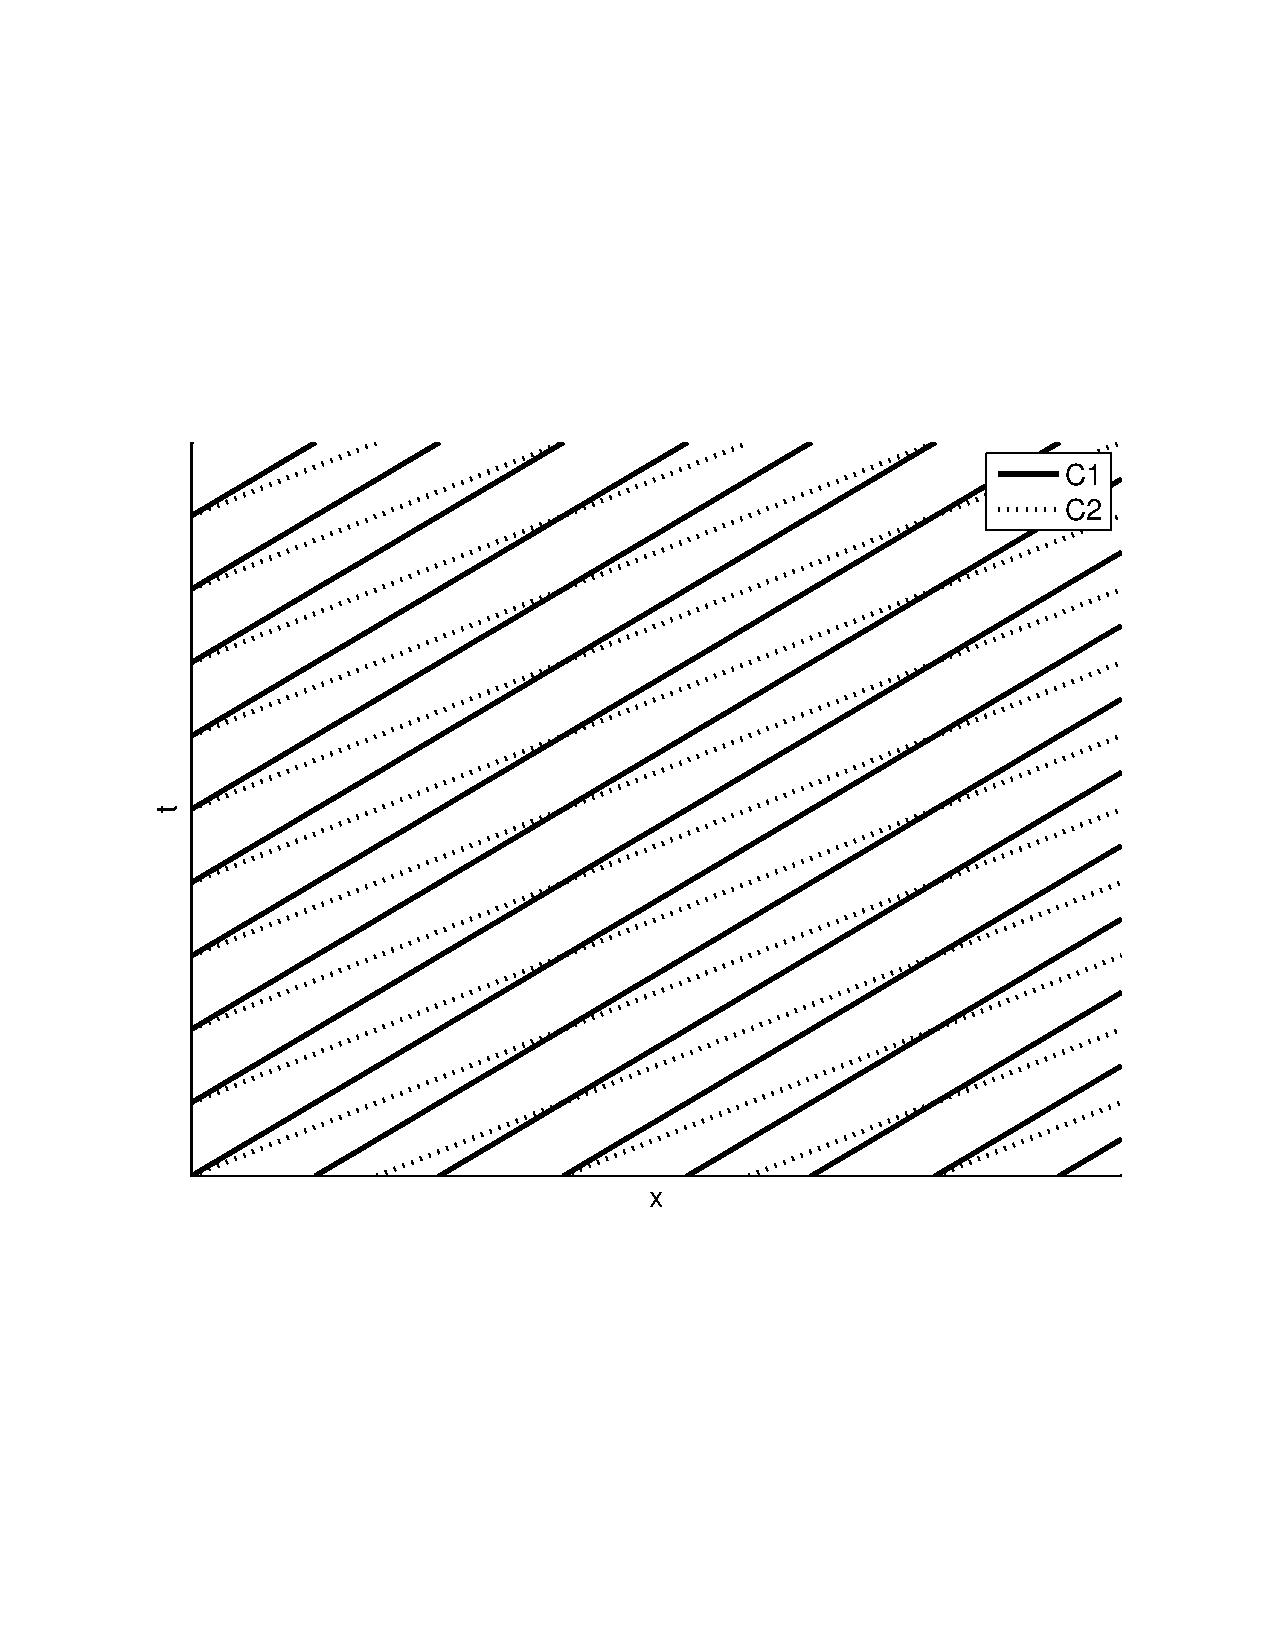
\includegraphics[trim= 0mm 75mm 0mm 70mm, width = 90mm]{supercr}
\caption{Illustration of the characteristics for supercritical flow, $\lambda_1 \geq \lambda_2 > 0$.}
\label{fig:supercr}
\end{figure}

With $\zeta_1 (0,t)$ and $\zeta_2 (0,t)$ as the inputs and $\zeta_1(L,t)$ and $\zeta_2(L,t)$ as the outputs, the distributed transfer matrix is exactly the state-transition matrix $\Phi(x,s)$.\\

Using \eqref{eq:Riemannzeta}, we can write

\begin{equation}
\begin{pmatrix}
\widetilde{v}(x,s) \\ \widetilde{q}(x,s)
\end{pmatrix} = \underbrace{ \begin{pmatrix}
\dfrac{\rho^*\lambda_2}{\lambda_1-\lambda_2} & 1\\
\dfrac{\rho^*\lambda_1}{\lambda_1-\lambda_2} & 0
\end{pmatrix}^{-1} \Phi(x,s) 
\begin{pmatrix}
\dfrac{\rho^*\lambda_2}{\lambda_1-\lambda_2} & 1\\
\dfrac{\rho^*\lambda_1}{\lambda_1-\lambda_2} & 0
\end{pmatrix} }_\text{$\Psi (x,s)$} \begin{pmatrix}
\widetilde{v}(0,s) \\ \widetilde{q}(0,s)
\end{pmatrix}
\end{equation}
with
\begin{subequations}
\begin{align}
\psi_{11}(x,s) &=\left(e^{-\frac{x}{\lambda_{1}\tau}}e^{-\frac{x}{\lambda_{1}}s}-e^{-\frac{x}{\lambda_{2}}s}\right)\frac{\alpha}{s+\alpha}+e^{-\frac{x}{\lambda_{2}}s}, \\
\psi_{12}(x,s)&=-\frac{1}{\rho^* \tau}\left(e^{-\frac{x}{\lambda_{1}\tau}}e^{-\frac{x}{\lambda_{1}}s}-e^{-\frac{x}{\lambda_{2}}s}\right)\frac{1}{s+\alpha}, \\
\psi_{21}(x,s)&=-\rho^{*} \tau\left(e^{-\frac{x}{\lambda_{1}\tau}}e^{-\frac{x}{\lambda_{1}}s}-e^{-\frac{x}{\lambda_{2}}s}\right)\frac{\alpha s}{s+\alpha}, \\
\psi_{22}(x,s)&=-\left(e^{-\frac{x}{\lambda_{1}\tau}}e^{-\frac{x}{\lambda_{1}}s}-e^{-\frac{x}{\lambda_{2}}s}\right)\frac{\alpha}{s+\alpha}+e^{-\frac{x}{\lambda_{1}\tau}}e^{-\frac{x}{\lambda_{1}}s}.
\end{align}
\end{subequations}

where $\alpha = -\dfrac{\lambda_2}{\tau(\lambda_1 - \lambda_2)}$. 

\subsubsection{Bode plots}

We generate Bode plots using the following parameters taken from \cite{Hofleitner}: $q_{max}$ = 1300 veh/h, $\rho_{max}$ = 0.1 veh/m, and $L$ = 100 m: The Greenshields Hamiltonian, $Q( \rho) = 4 \frac{q_{max}}{\rho_{max}^2}\rho (\rho_{max} - \rho)$, is used to approximate the fundamental diagram. For inhomogenous second-order models, the relaxation time, $\tau$, falls in the range of about 14-60 seconds \cite{Fan}. A relaxation time of $\tau$ = 15 s is used for the following simulations. We simulate for $\rho^* = 0.01$. \\

For the physical variables: 
\begin{figure}[H]
\centering
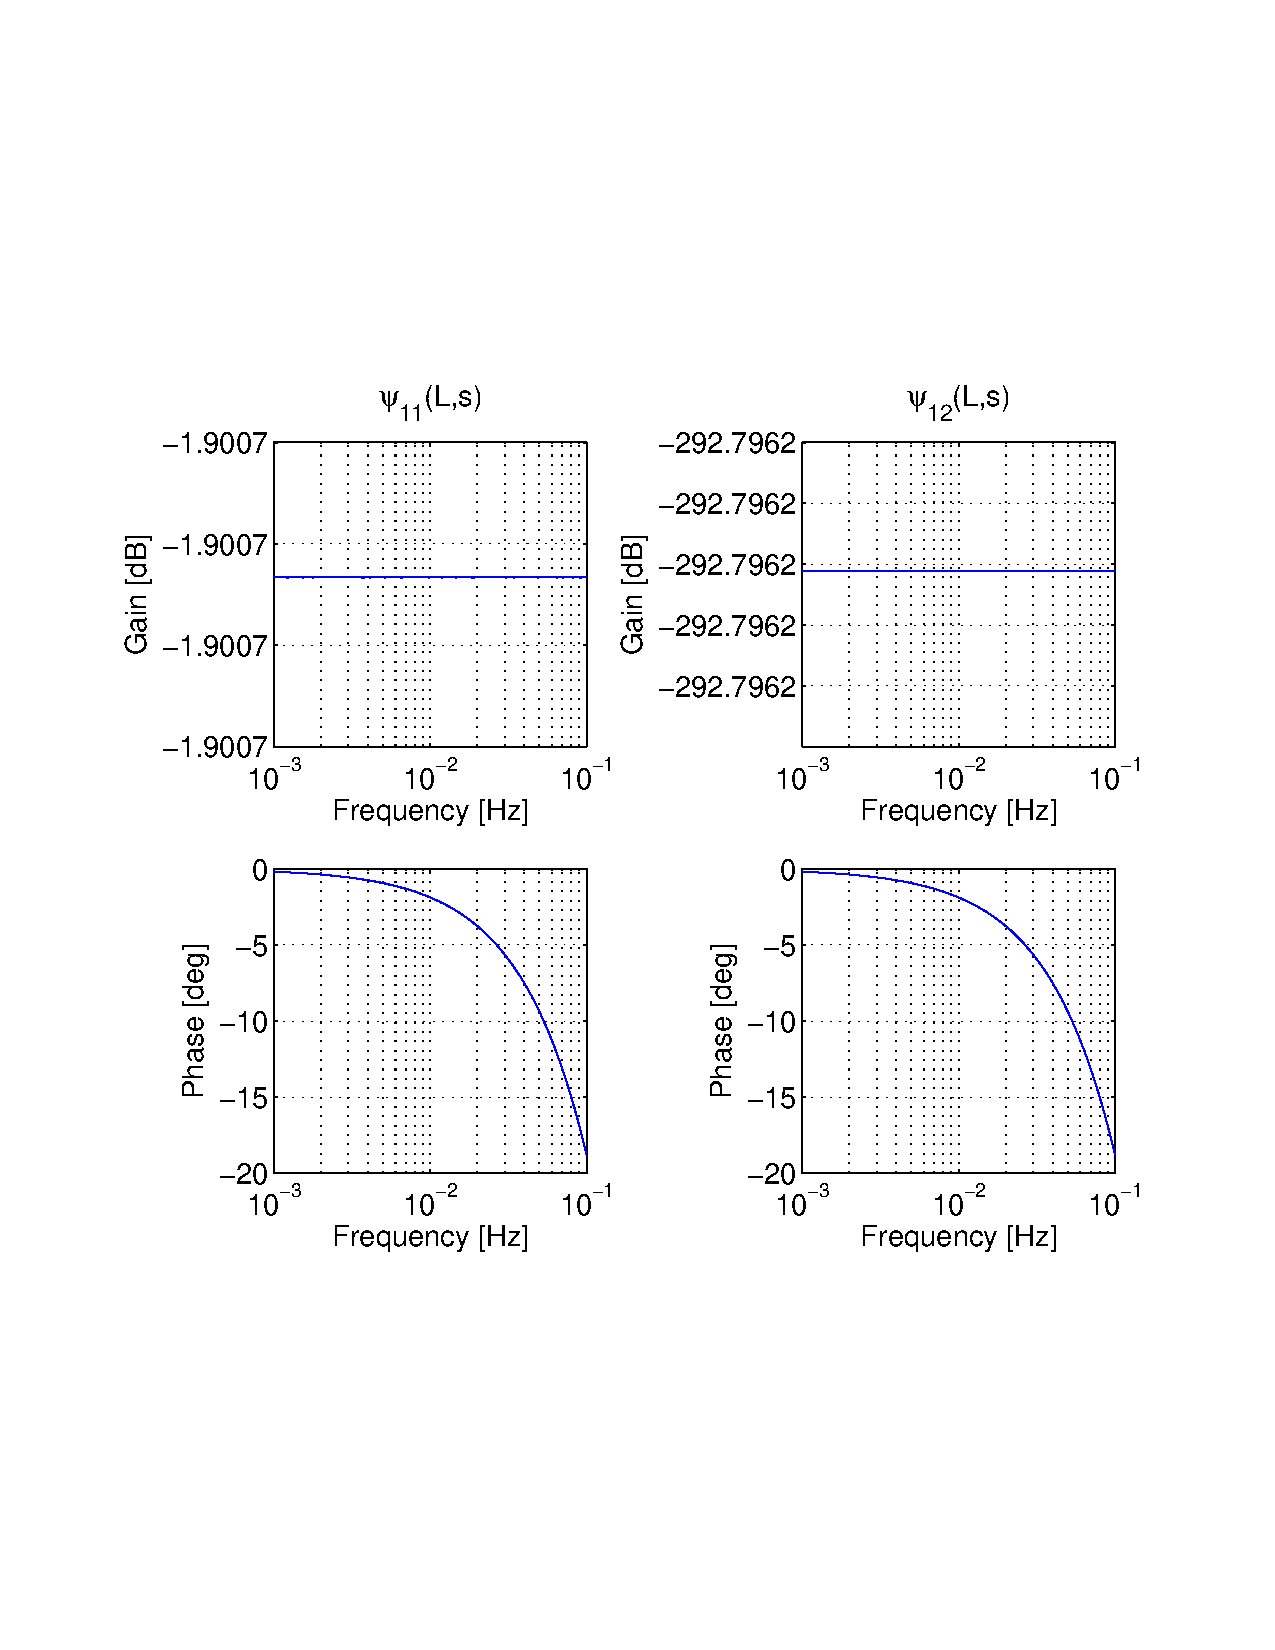
\includegraphics[trim = 0mm 60mm 0mm 60mm, width = 110mm]{IOv_-3to-1}
\caption{Bode magnitude and phase plots for $\psi_{11}(L,s)$ and $\psi_{12}(L,s)$.}
\end{figure}

\begin{figure}[H]
\centering
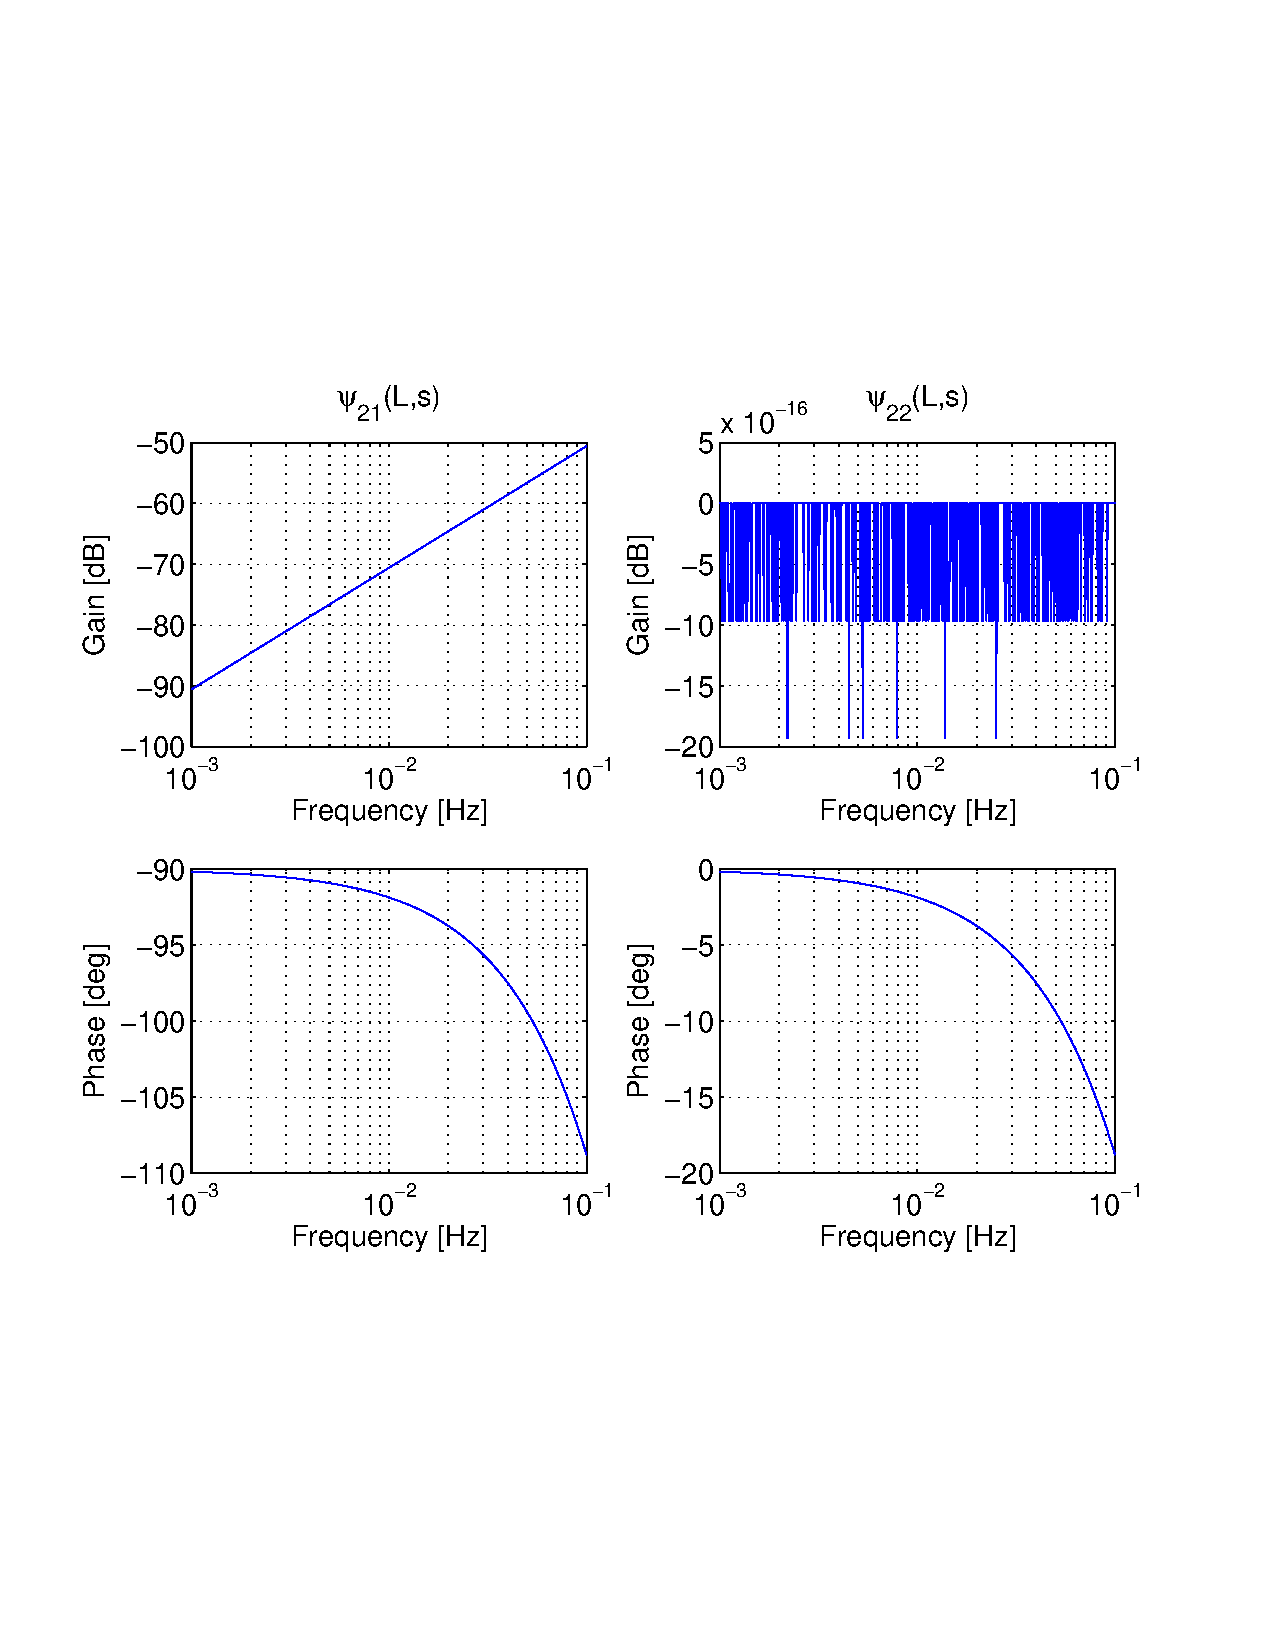
\includegraphics[trim = 0mm 60mm 0mm 60mm, width = 110mm]{IOq_-3to-1}
\caption{Bode magnitude and phase plots for $\psi_{21}(L,s)$ and $\psi_{22}(L,s)$.}
\end{figure}

\begin{figure}[H]
\centering
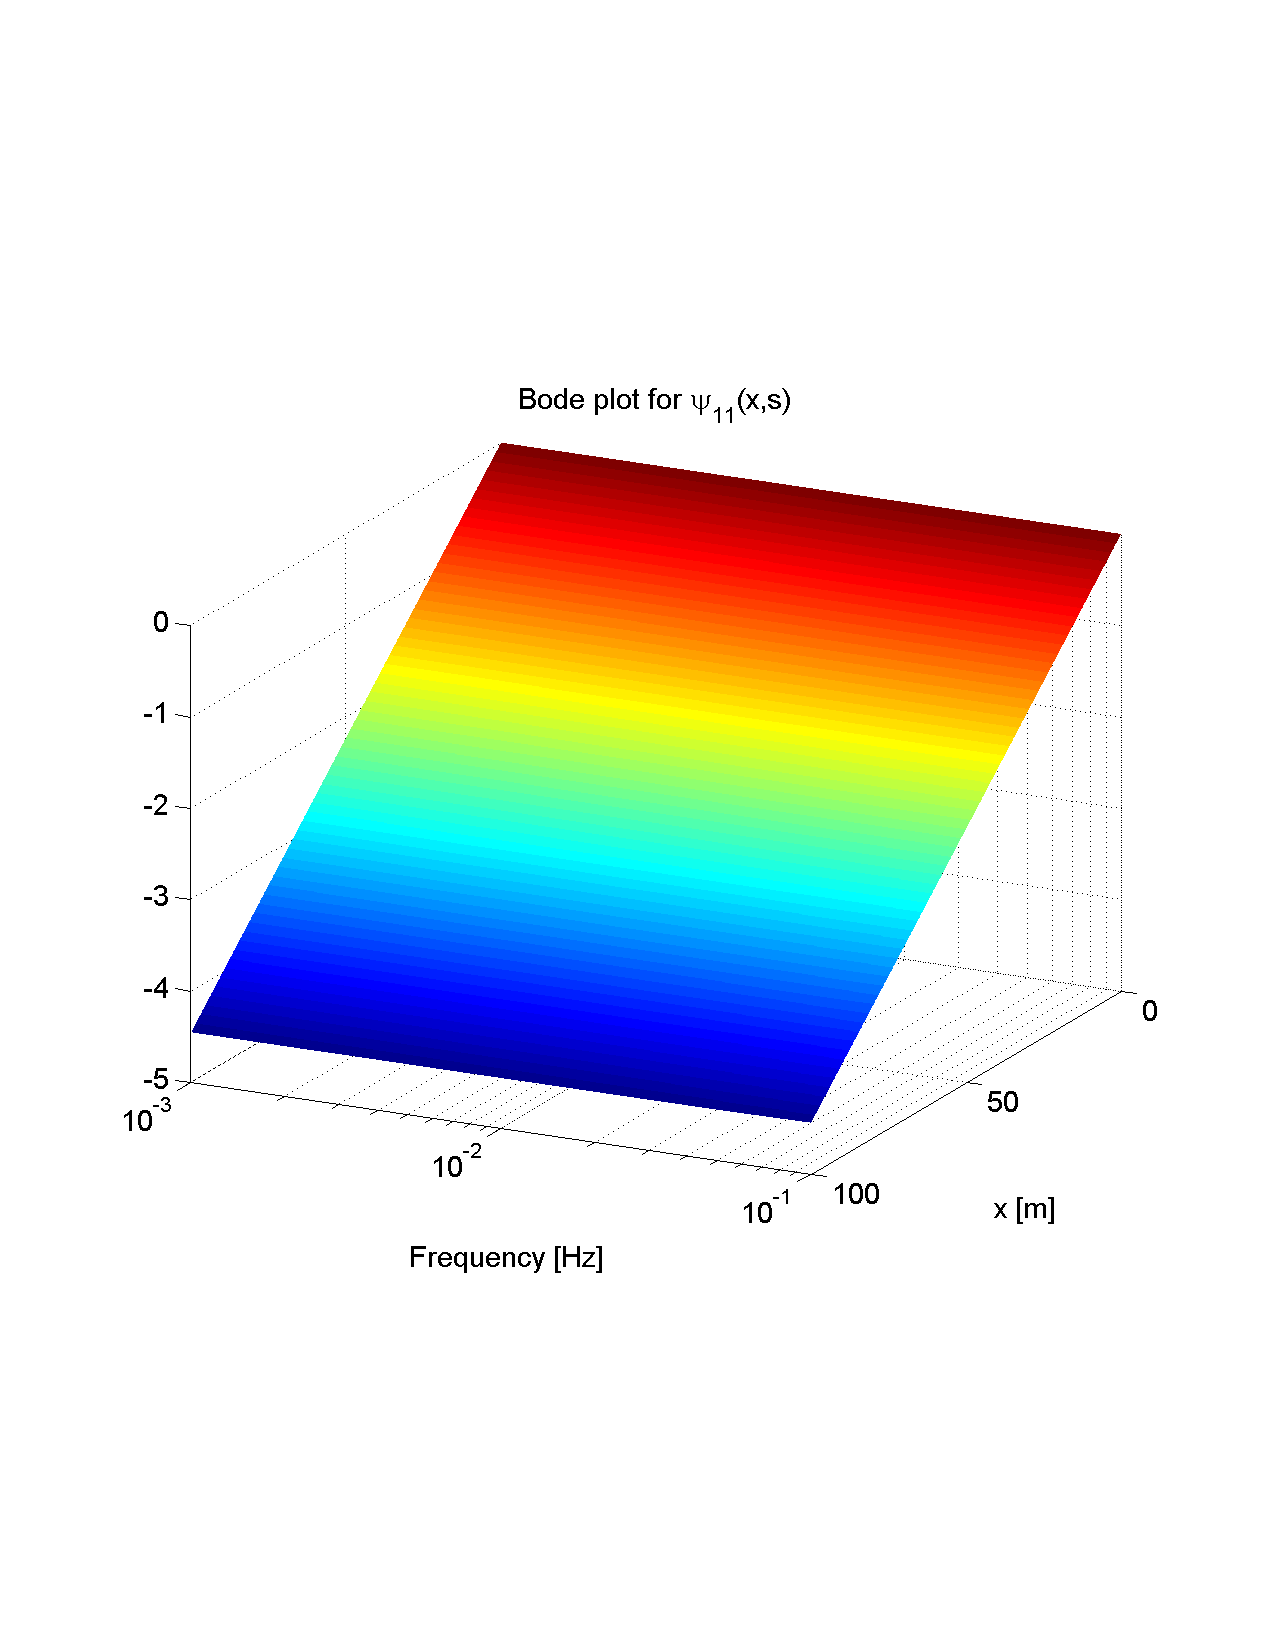
\includegraphics[trim = 0mm 60mm 0mm 60mm, width = 120mm]{distr11_-3to-1}
\caption{Spatial Bode magnitude plot for $\psi_{11}(x,s)$.}
\end{figure}


\begin{figure}[H]
\centering
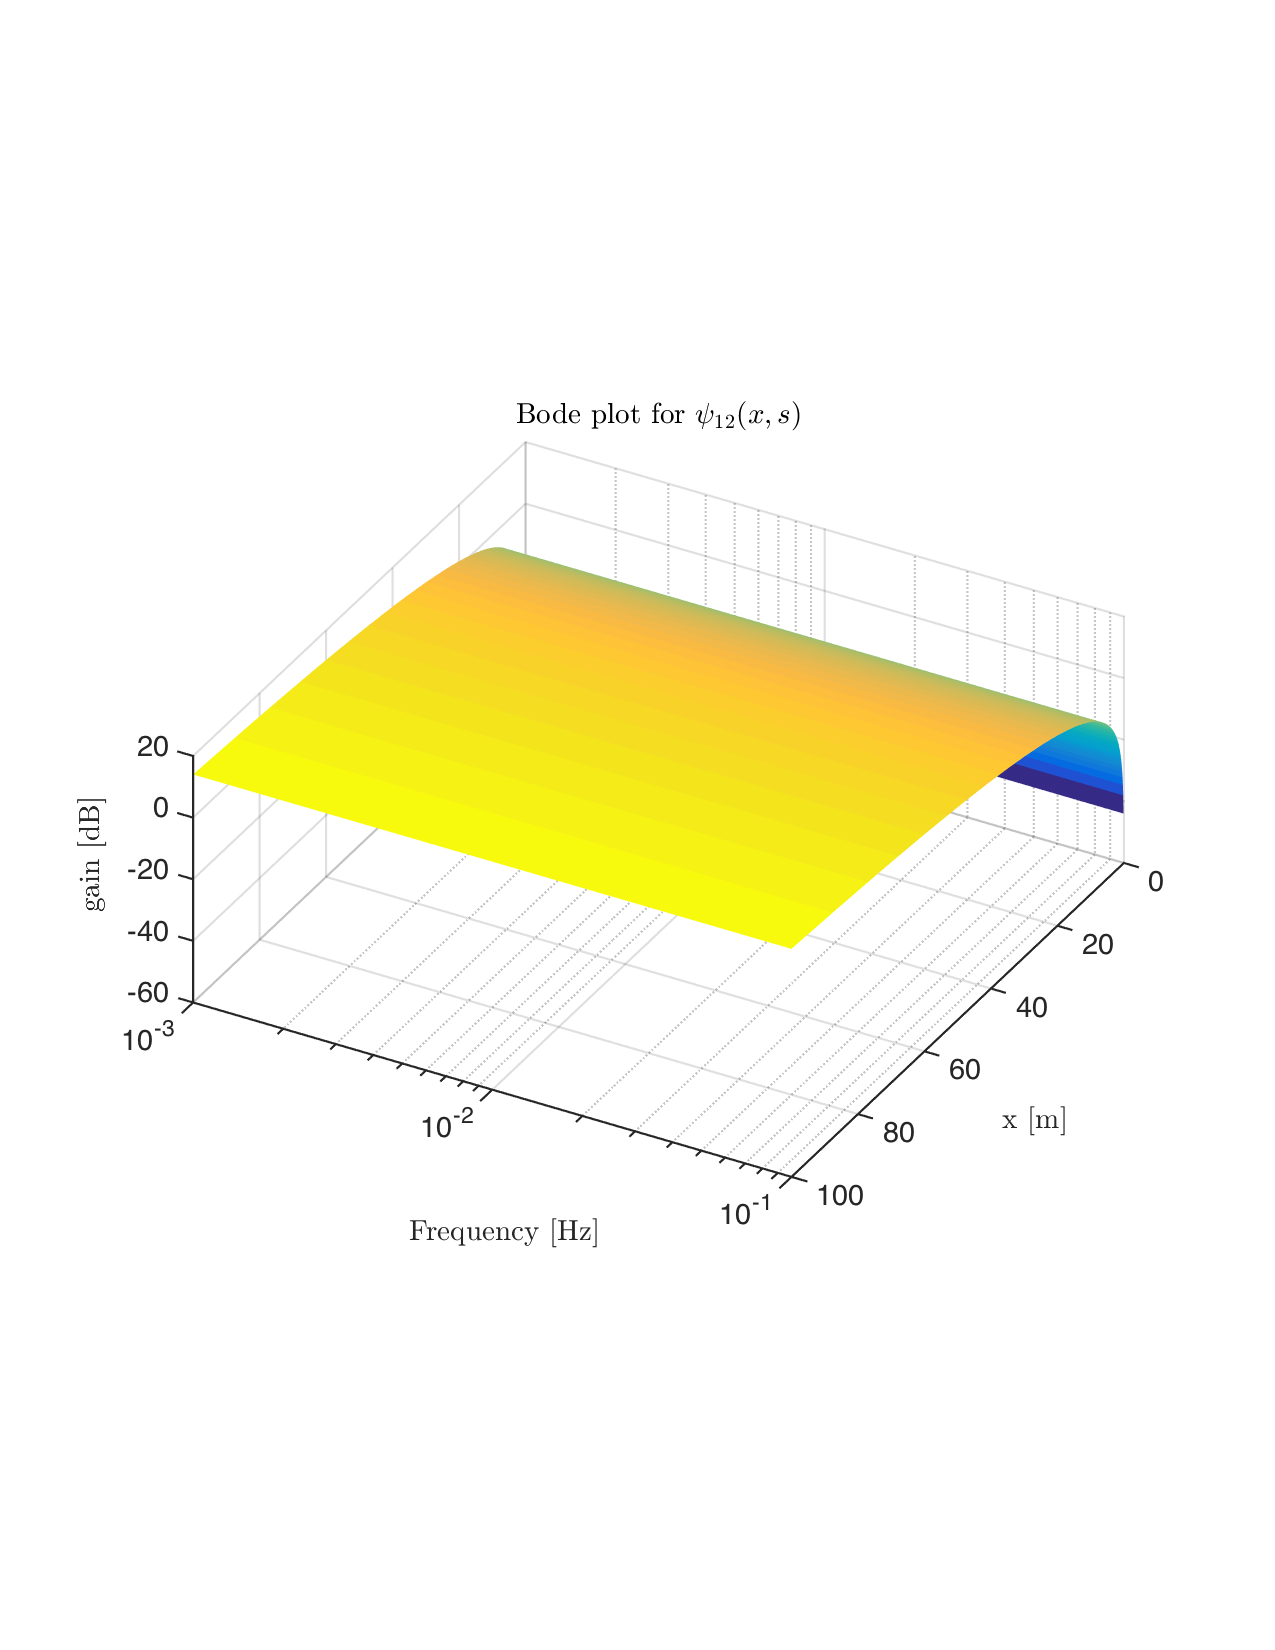
\includegraphics[trim = 0mm 60mm 0mm 60mm, width = 120mm]{distr12_-3to-1}
\caption{Spatial Bode magnitude plot for $\psi_{12}(x,s)$.}
\end{figure}

\begin{figure}[H]
\centering
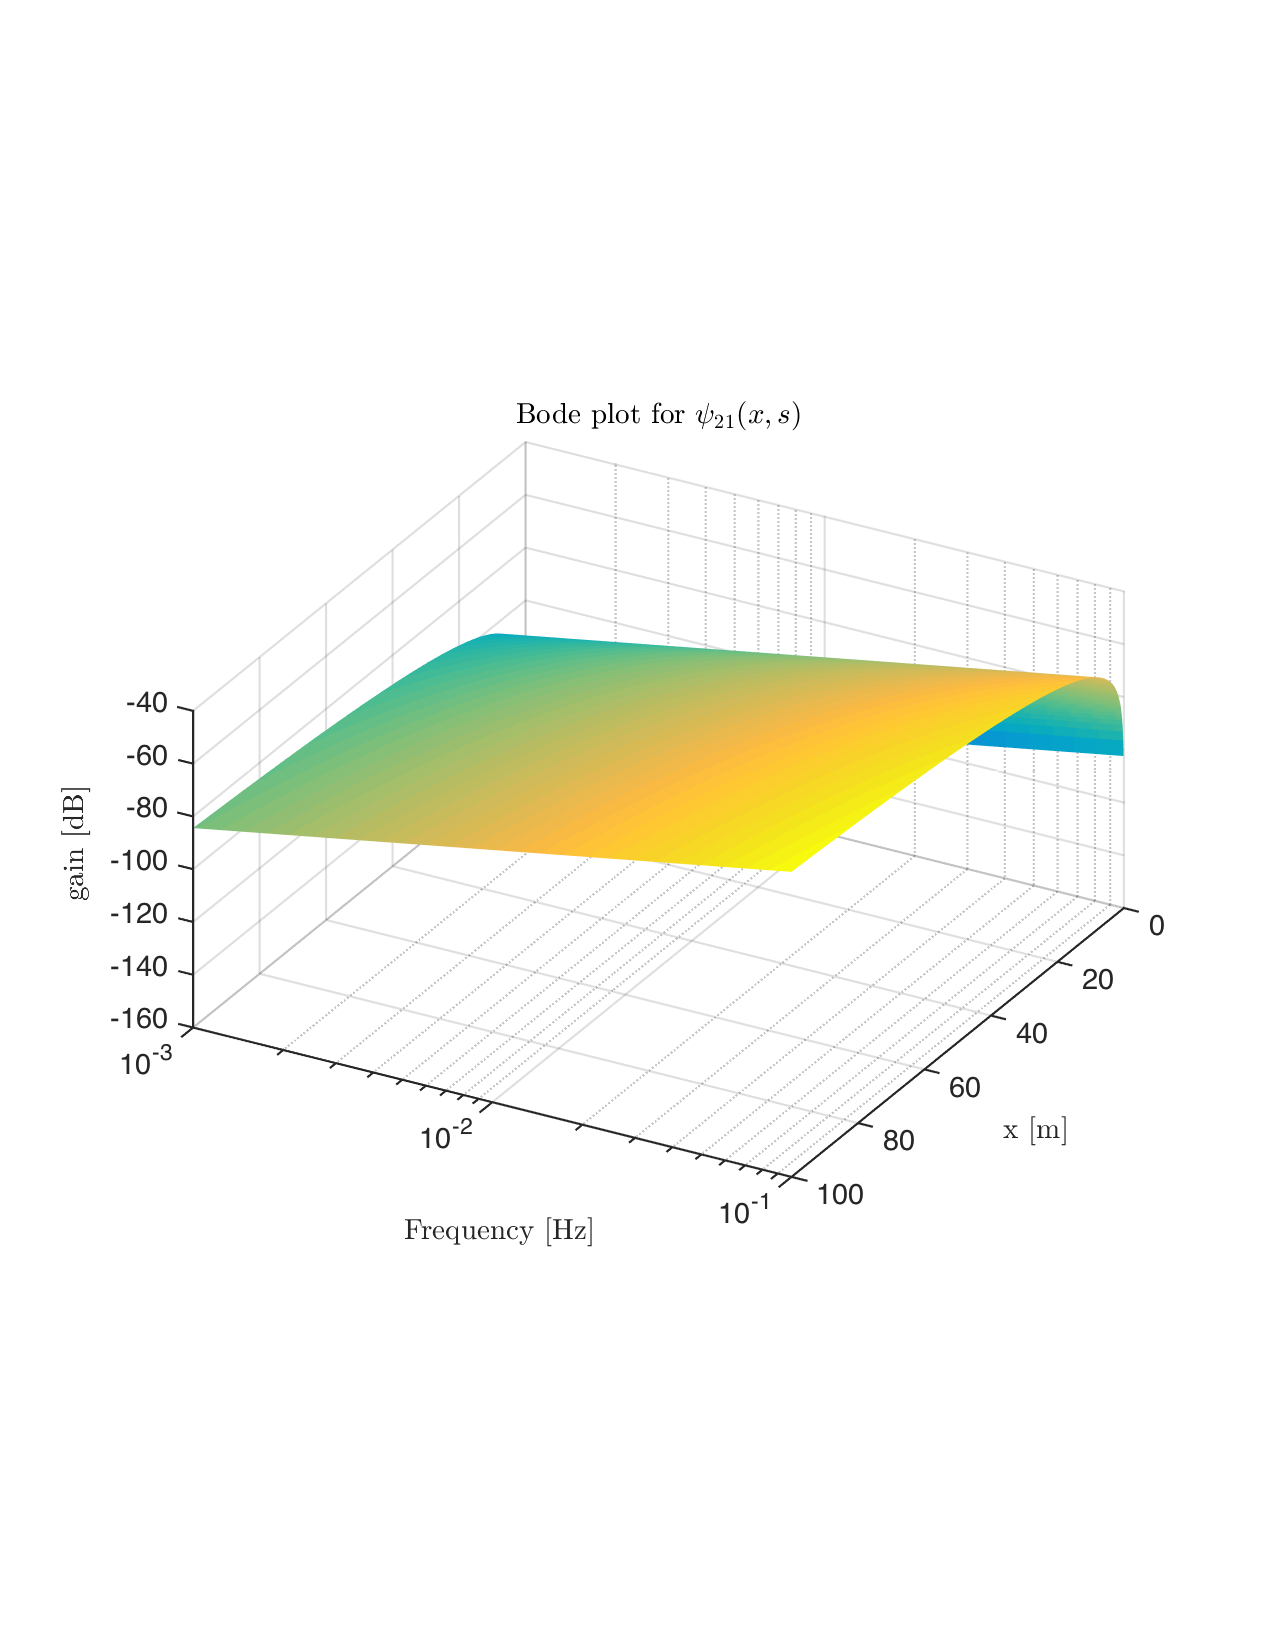
\includegraphics[trim = 0mm 60mm 0mm 60mm, width = 120mm]{distr21_-3to-1}
\caption{Spatial Bode magnitude plot for $\psi_{21}(x,s)$.}
\end{figure}

\begin{figure}[H]
\centering
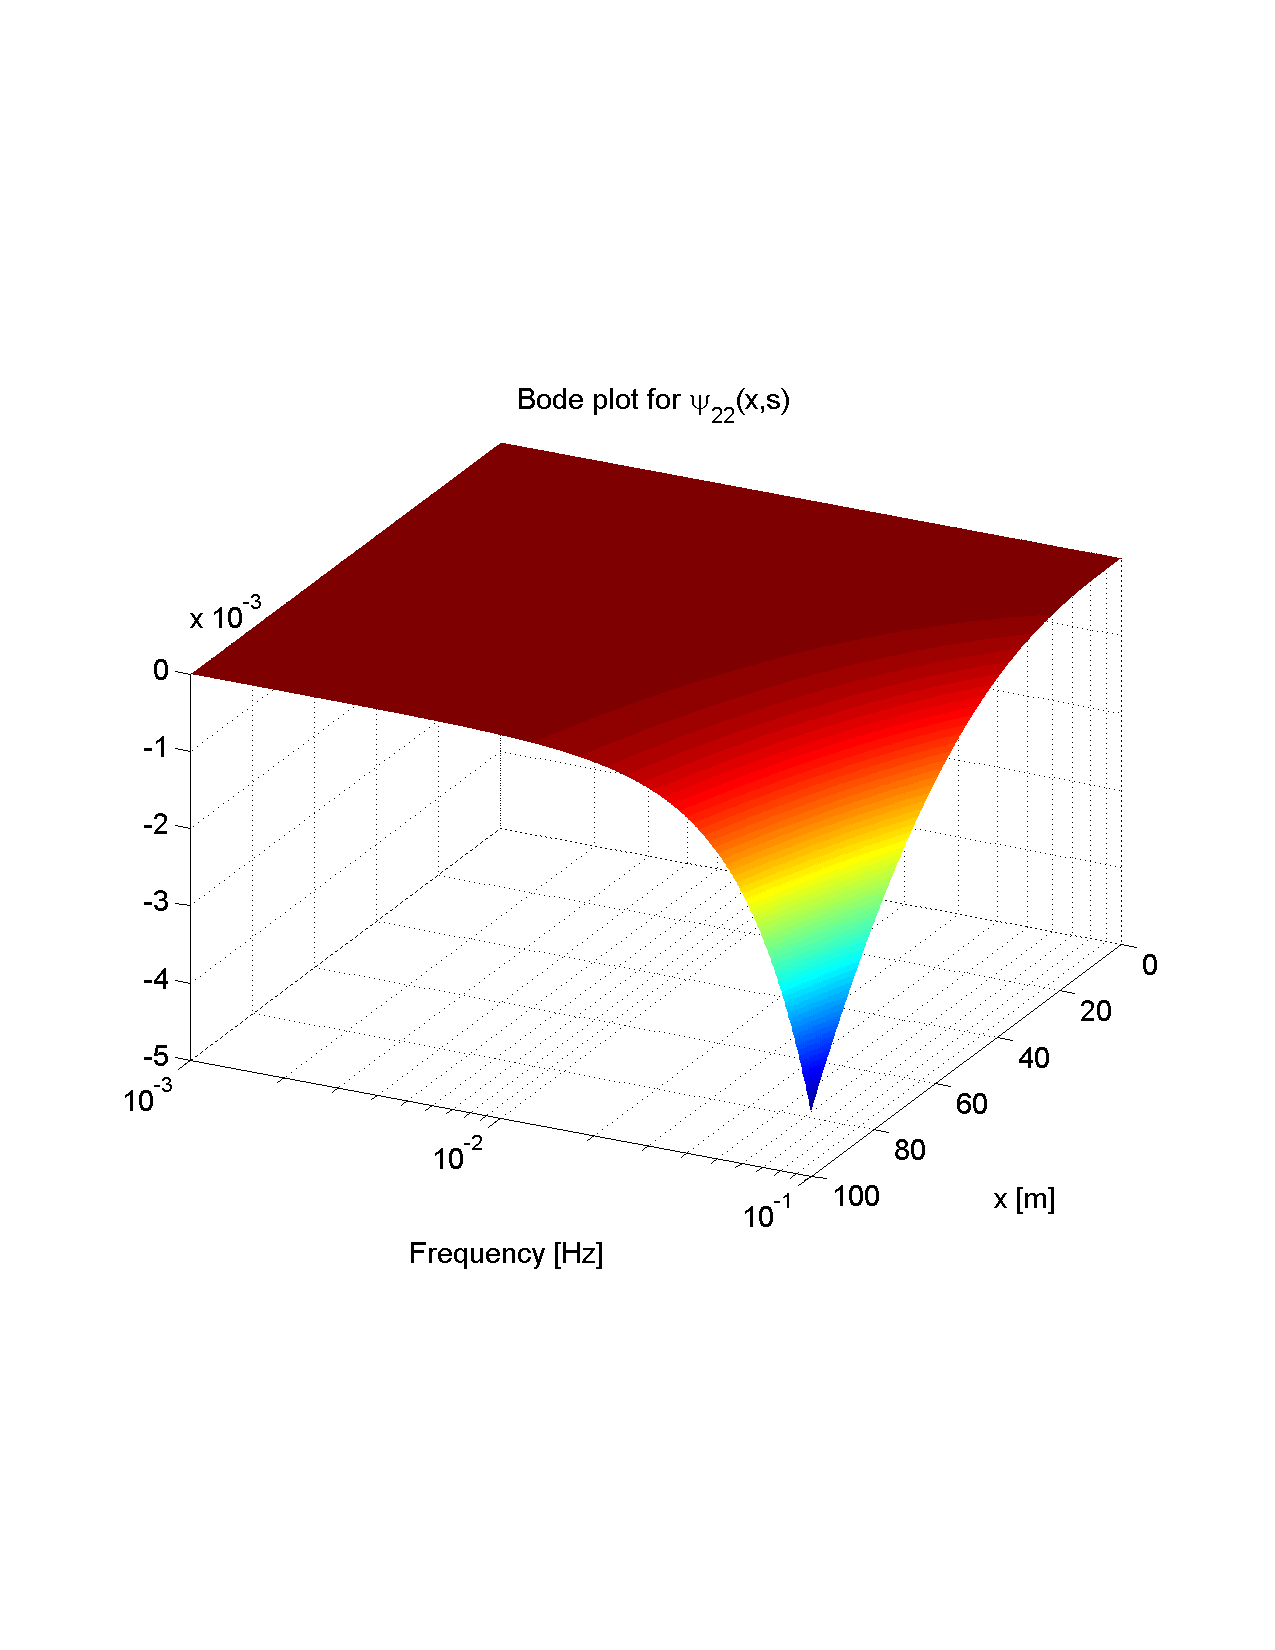
\includegraphics[trim = 0mm 60mm 0mm 60mm, width = 120mm]{distr22_-3to-1}
\caption{Spatial Bode magnitude plot for $\psi_{22}(x,s)$.}
\end{figure}
\clearpage

For the Riemann invariants: 
\begin{figure}[H]
\centering
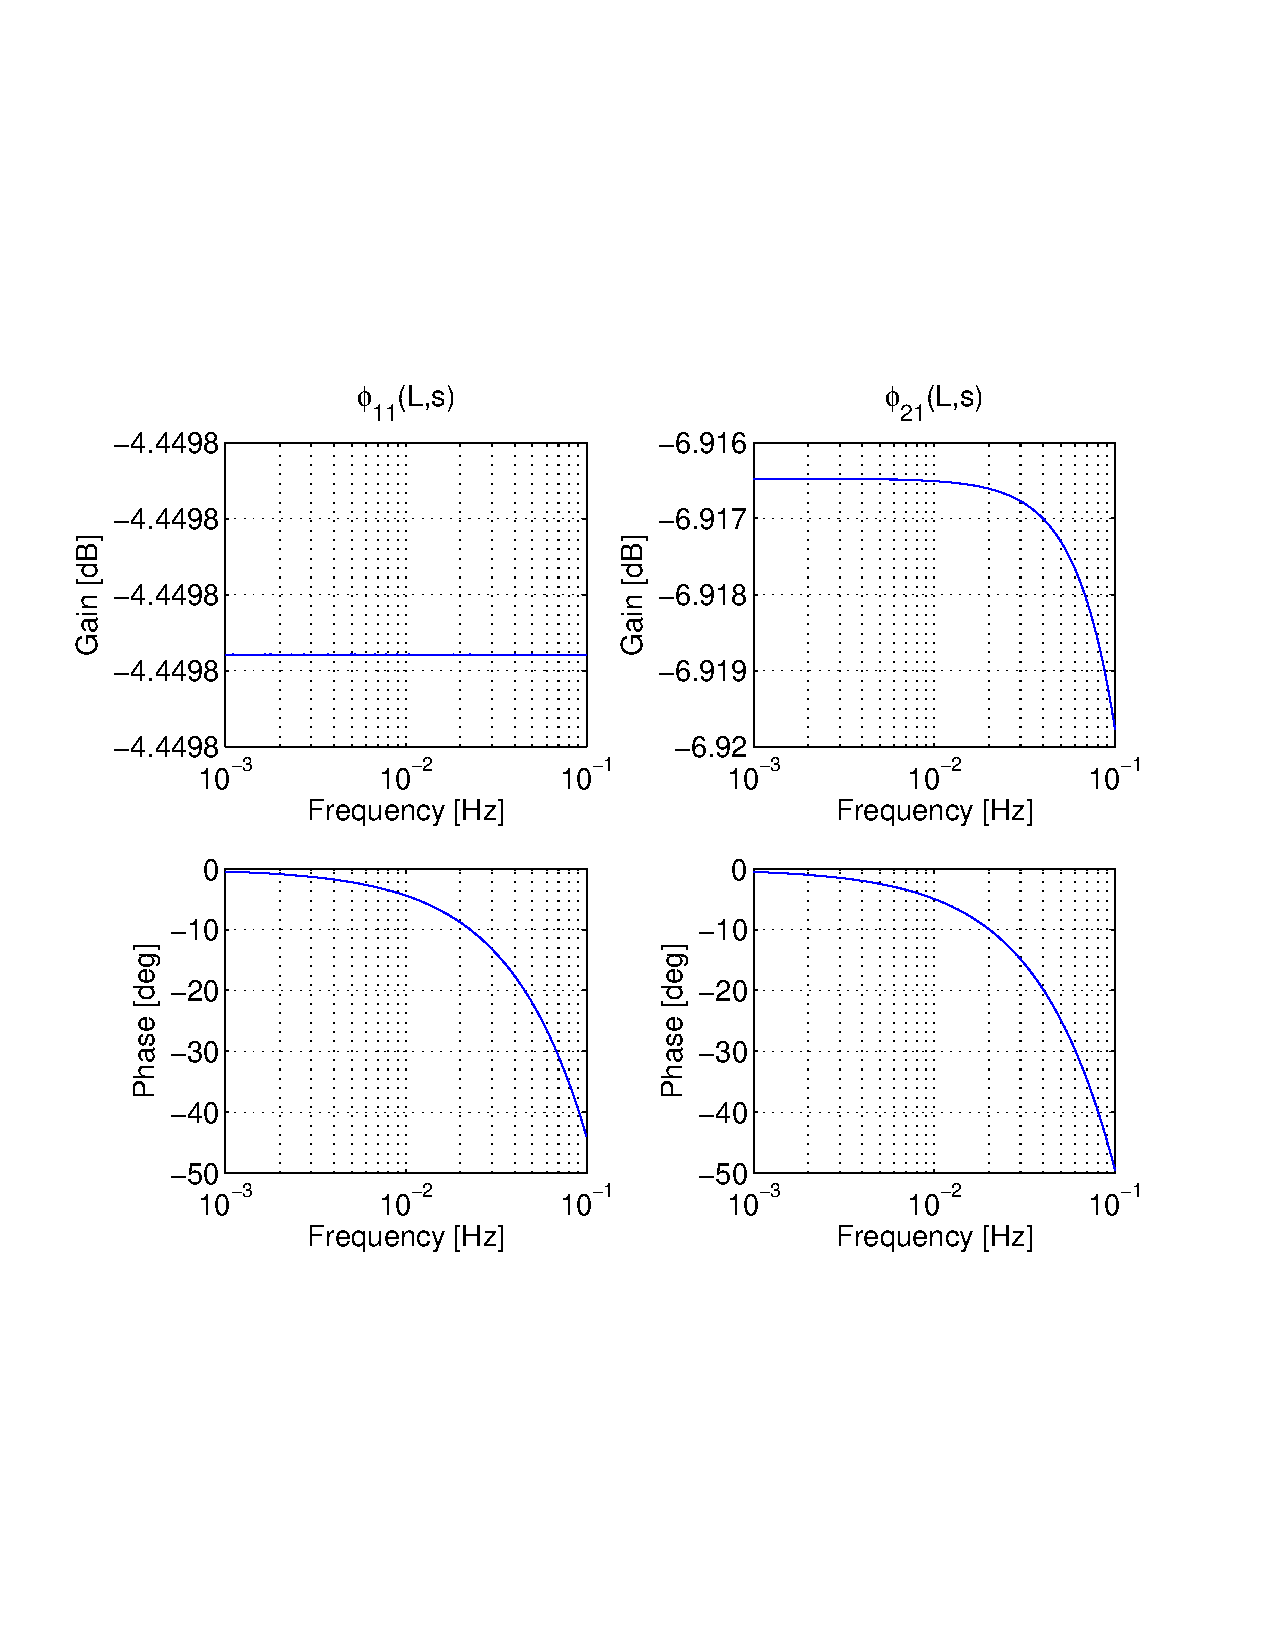
\includegraphics[trim = 0mm 60mm 0mm 60mm, width = 110mm]{diagIOfreeflow}
\caption{Bode magnitude and phase plots for $\phi_{11}(L,s)$ and $\phi_{21}(L,s)$.}
\end{figure}

\begin{figure}[H]
\centering
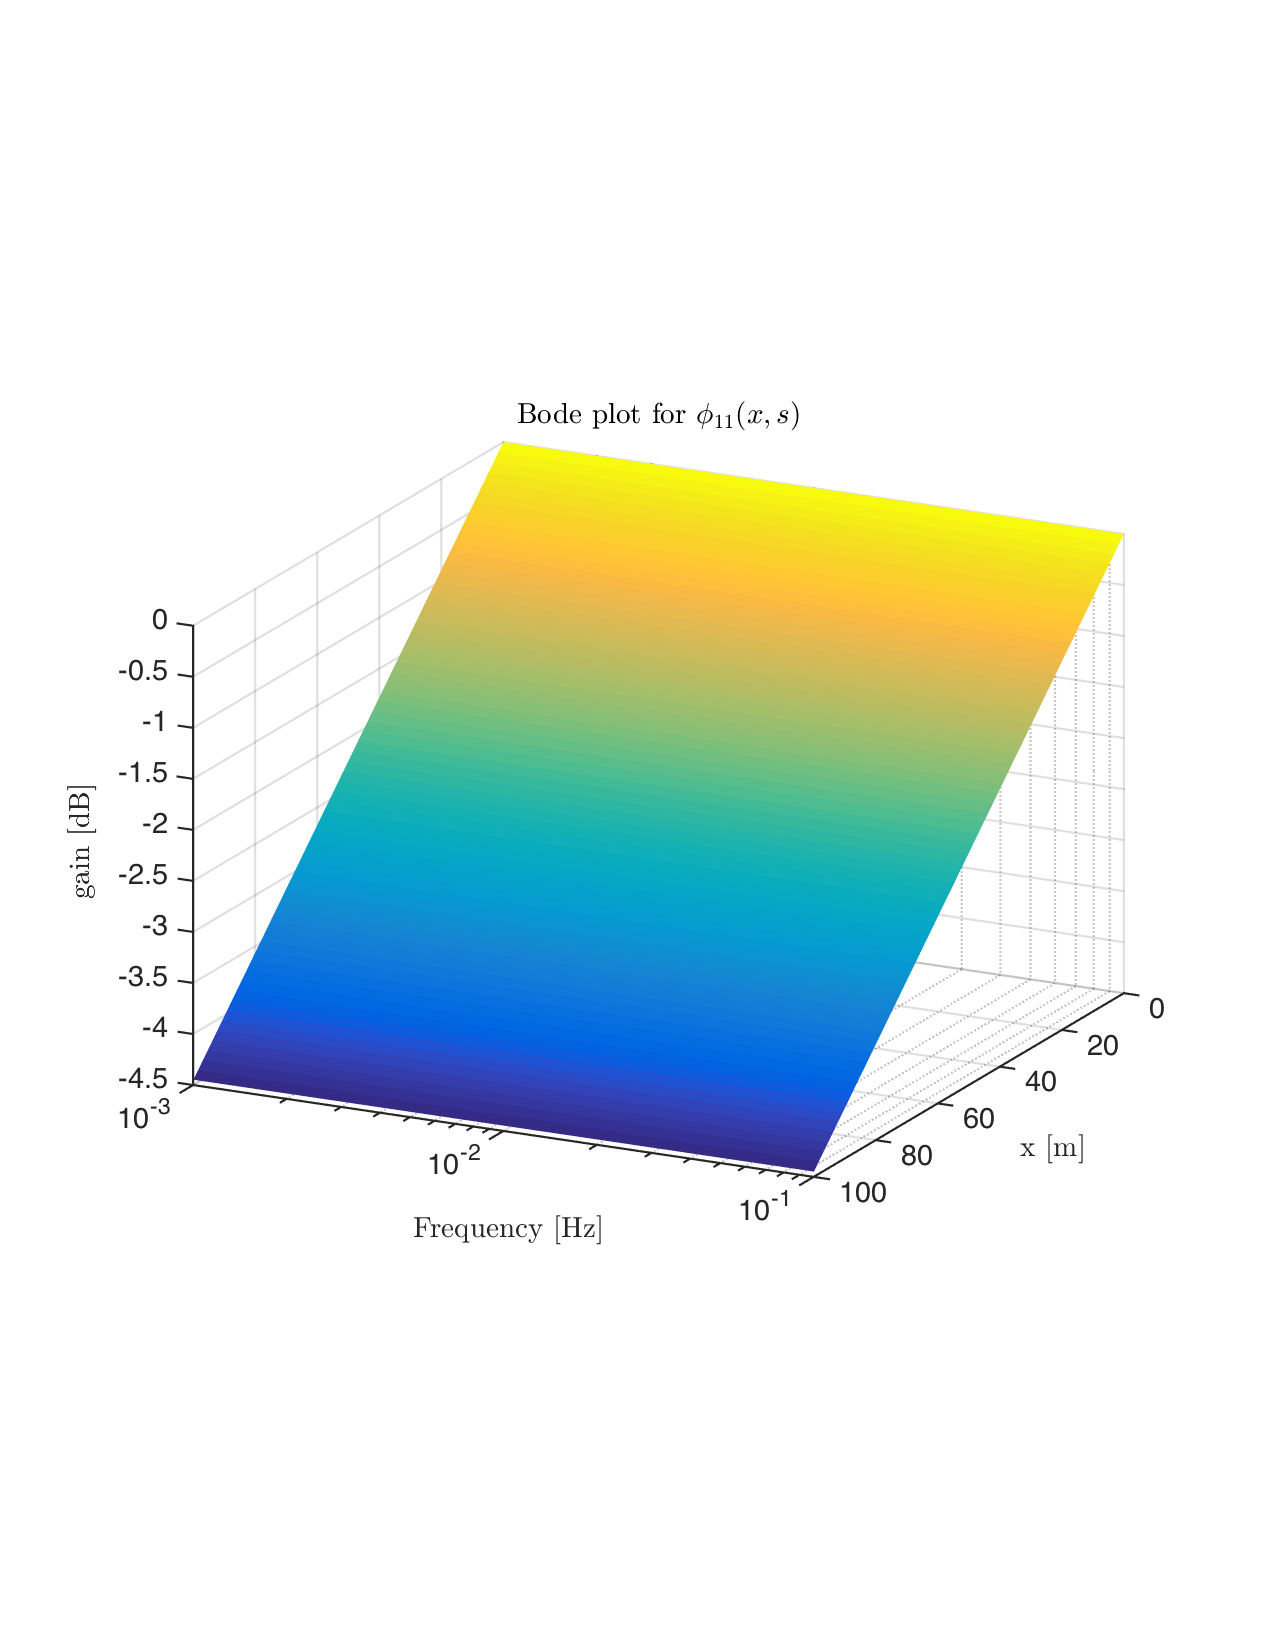
\includegraphics[trim = 0mm 60mm 0mm 60mm, width = 120mm]{diagdistr11freeflow}
\caption{Spatial Bode magnitude plot for $\phi_{11}(x,s)$.}
\end{figure}
\clearpage
\begin{figure}[H]
\centering
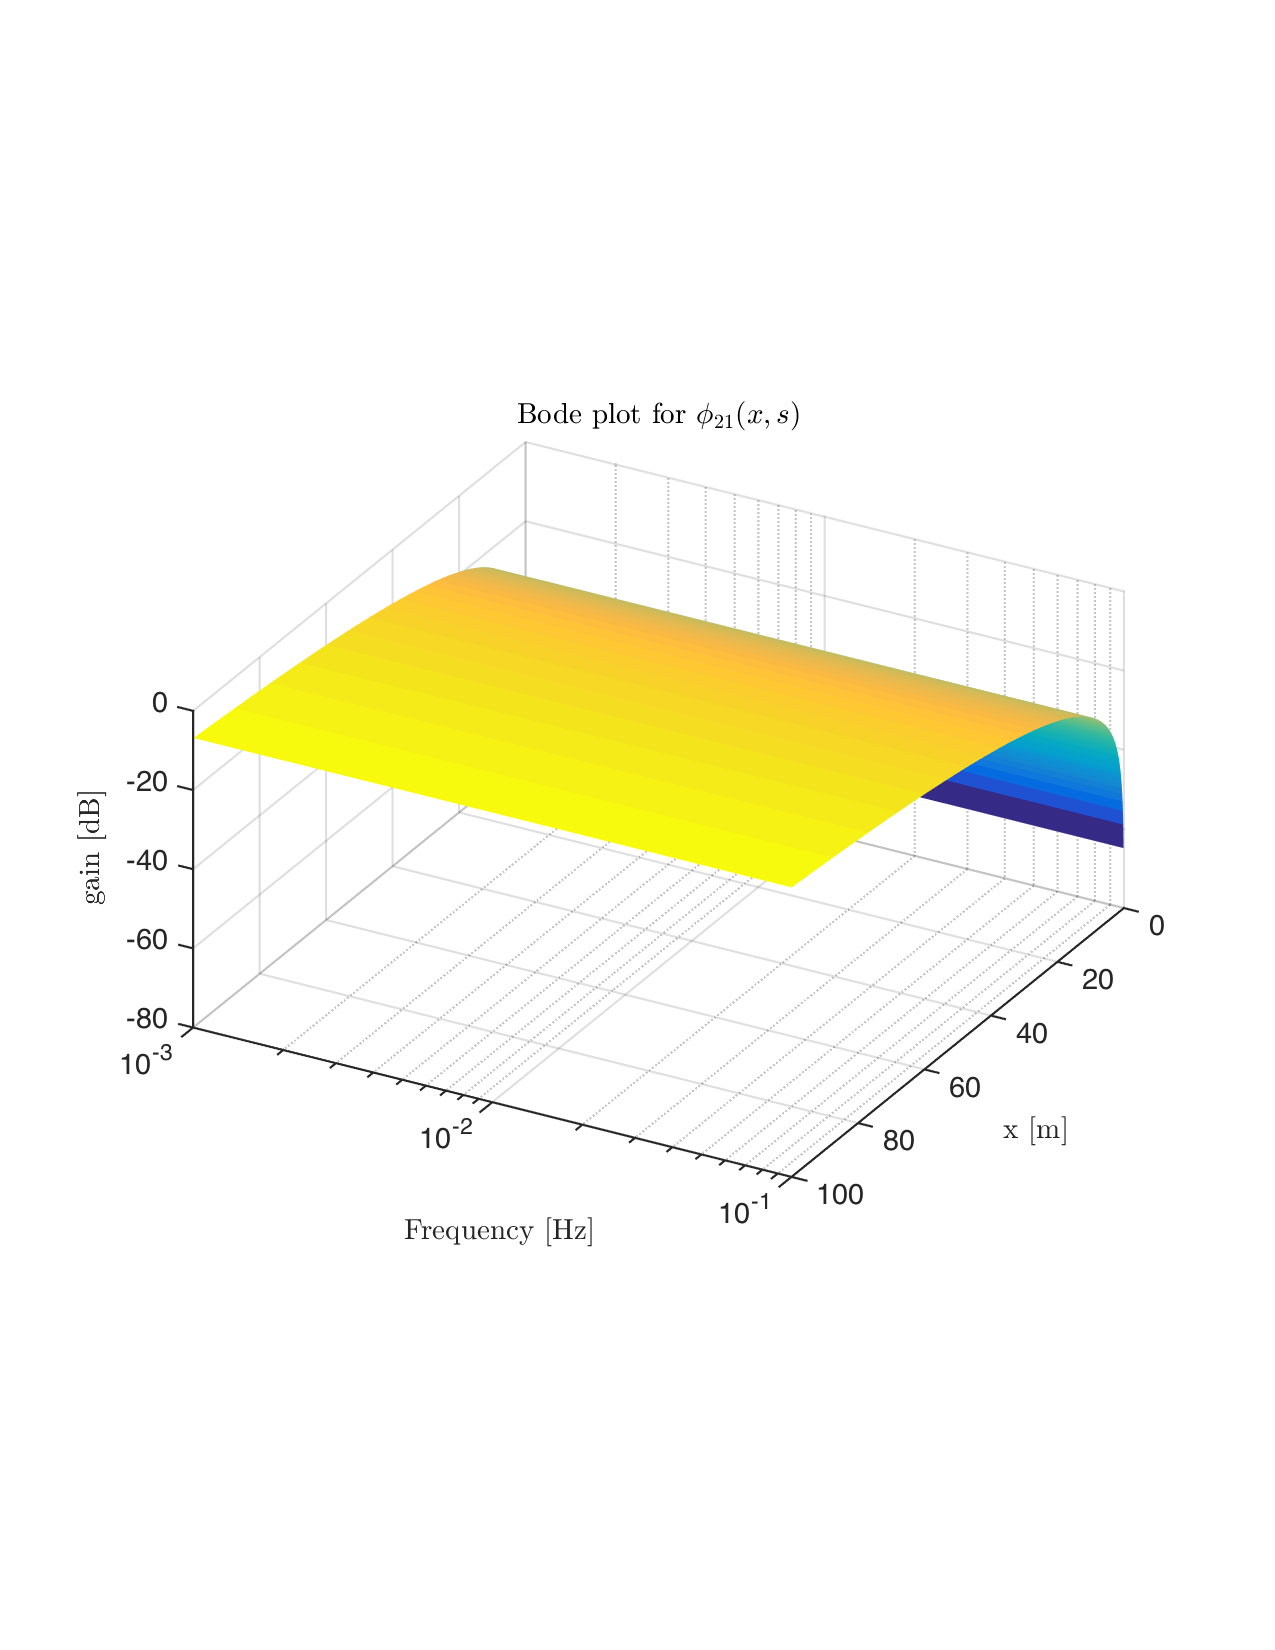
\includegraphics[trim = 0mm 60mm 0mm 60mm, width = 120mm]{diagdistr21freeflow}
\caption{Spatial Bode magnitude plot for $\phi_{21}(x,s)$.}
\end{figure}


\subsubsection{Step responses}
We analyze the behavior of the system given step inputs $v(0,t)=v_{step}H(t)$ and $q(0,t)=q_{step}H(t)$, where $H(\cdot)$ is the Heaviside function. The step responses are

\begin{align} 
v(x,t) &= v_{step}\left[e^{-\frac{x}{\lambda_1\tau}}\left(1 - e^{-a\left(t-\frac{x}{\lambda_1}\right)}\right)H\left(t-\frac{x}{\lambda_1}\right) + e^{-a\left(t-\frac{x}{\lambda_2}\right)}H\left(t-\frac{x}{\lambda_2}\right)\right] \notag \\
&\quad+ \dfrac{q_{step}}{\rho^* \tau}\left[- e^{-\frac{x}{\lambda_1\tau}}\left(1 - e^{-a\left(t-\frac{x}{\lambda_1}\right)}\right)H\left(t-\frac{x}{\lambda_1}\right) + \left(1 - e^{-a\left(t-\frac{x}{\lambda_2}\right)}\right)H\left(t-\frac{x}{\lambda_2}\right) \right] \\
q(x,t) &= v_{step}\rho^*\tau a\left[e^{-\frac{x}{\lambda_1\tau}}e^{-a\left(t-\frac{x}{\lambda_1}\right)}H\left(t-\frac{x}{\lambda_1}\right) - e^{-a\left(t-\frac{x}{\lambda_2}\right)}H\left(t-\frac{x}{\lambda_2}\right) \right] \notag \\
&\quad+ q_{step}\left[ e^{-\frac{x}{\lambda_1\tau}}e^{-a\left(t-\frac{x}{\lambda_1}\right)}H\left(t-\frac{x}{\lambda_1}\right) + \left(1 - e^{-a\left(t-\frac{x}{\lambda_2}\right)}\right)H\left(t-\frac{x}{\lambda_2}\right)\right]
\end{align}


\subsection{Congested flow}
Consider now the system in the congestion flow regime. Here we have $\lambda_1 > 0, \lambda_2 < 0$, hence two boundary conditions are needed, one at the upstream boundary and one at the downstream boundary. A plot of the characteristics is shown in Figure \ref{fig:subcr}. \\

\begin{figure}[H] 
\centering
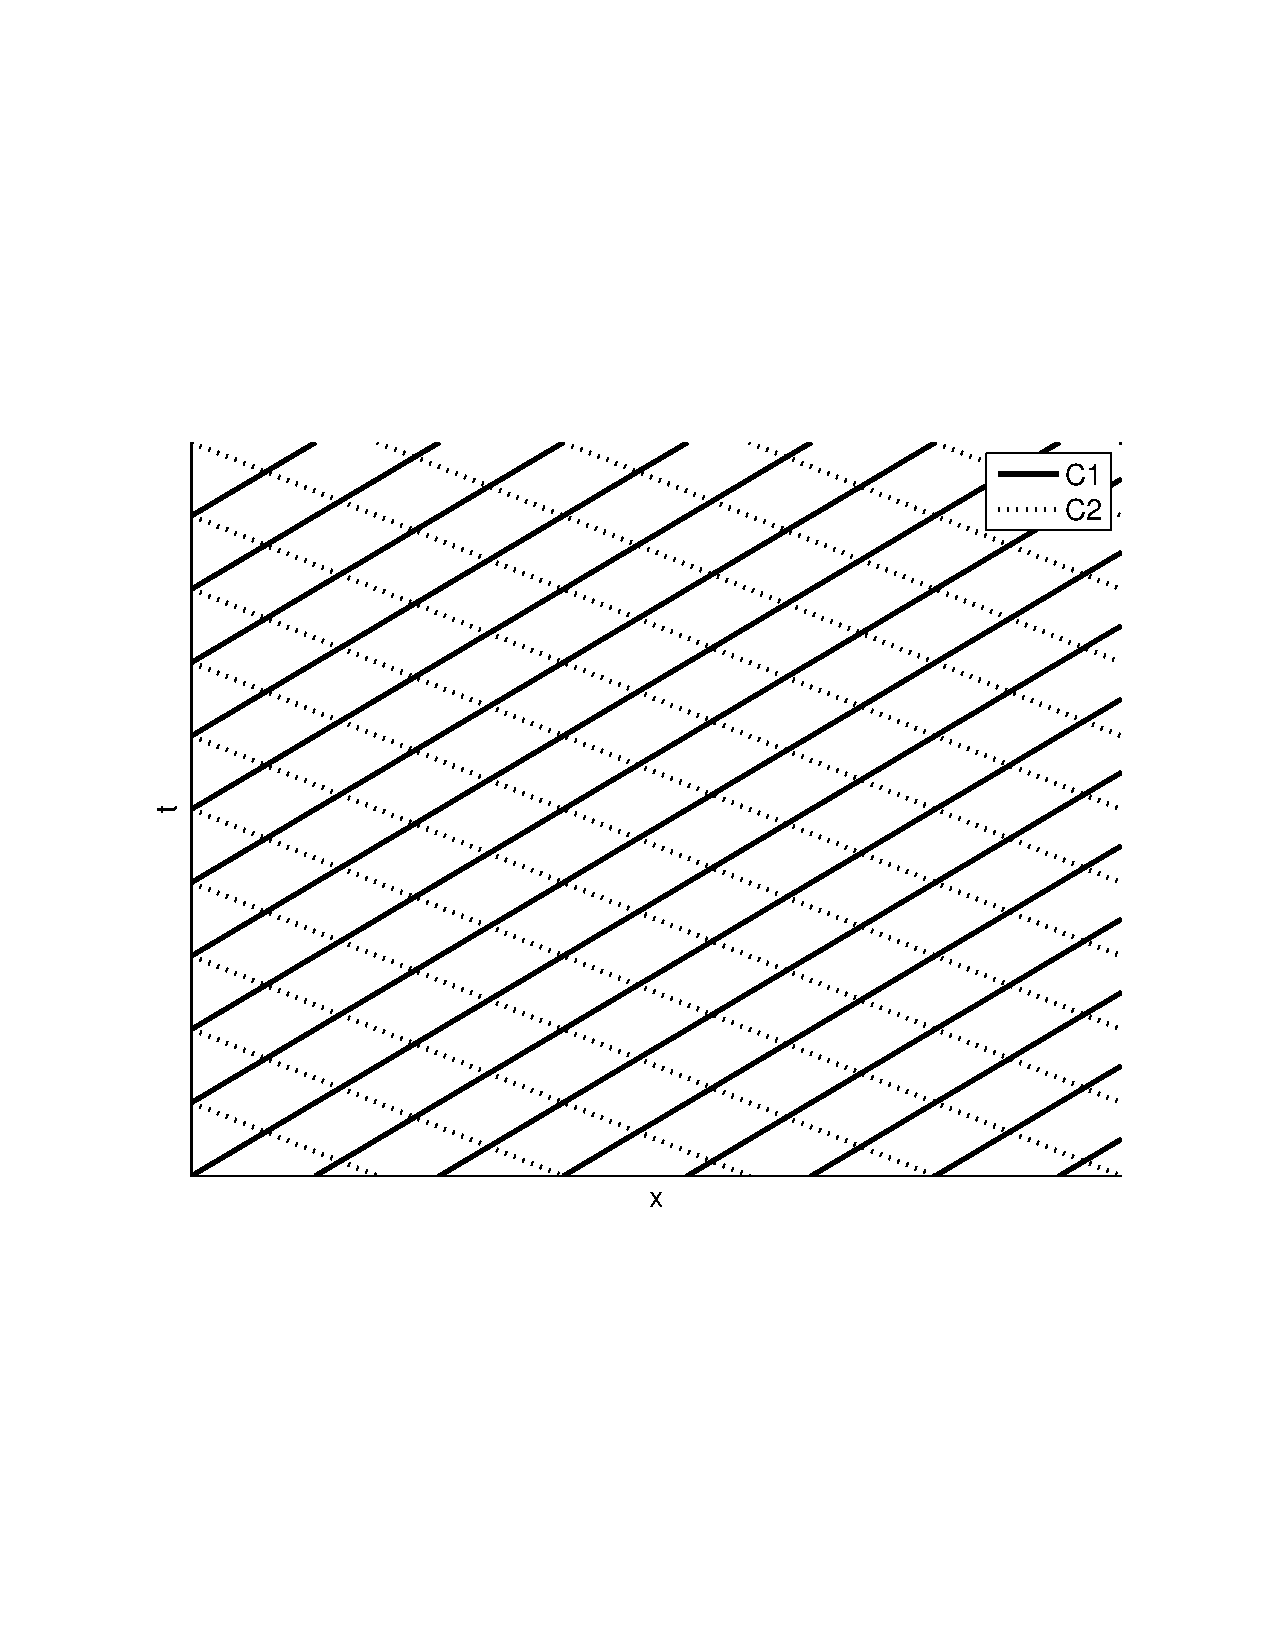
\includegraphics[trim= 0mm 75mm 0mm 70mm, width = 90mm]{subcr}
\caption{Illustration of the characteristics for supercritical flow, $\lambda_1 > 0, \lambda_2 < 0$.}
\label{fig:subcr}
\end{figure}


Using \eqref{TFRiemann} we can write 
\begin{equation}
\begin{pmatrix}
\hat{\xi_{1}}(x,s)\\
\hat{\xi_{2}}(x,s)
\end{pmatrix} = \underbrace{
\Phi(x,s) \begin{pmatrix}
1 & 0\\
-\frac{\phi_{21}\left(L,s\right)}{\phi_{22}\left(L,s\right)} & \frac{1}{\phi_{22}}
\end{pmatrix}}_\text{$\Gamma (x,s)$}
\begin{pmatrix}
\hat{\xi_{1}}\left(0,s\right)\\
\hat{\xi_{2}}\left(0,s\right)
\end{pmatrix}.
\end{equation}
with 
\begin{subequations}
\begin{align}
\gamma_{11}\left(x,s\right)&=e^{-\frac{x}{\lambda_{1}\tau}}e^{-\frac{sx}{\lambda_{1}}}, \\
\gamma_{12}\left(x,s\right)&=0, \\
\gamma_{21}\left(x,s\right)&=\alpha\frac{\lambda_{1}}{\lambda_{2}}\left(e^{-\frac{x}{\lambda_{1}\tau}}e^{-\frac{sx}{\lambda_{1}}}-e^{-\frac{L}{\lambda_{1}\tau}}e^{-\frac{s}{\lambda_{2}}\left(x-L\frac{\lambda_{1}-\lambda_{2}}{\lambda_{1}}\right)}\right)\frac{1}{s+\alpha}, \\
\gamma_{22}\left(x,s\right)&=e^{-\frac{s\left(x-L\right)}{\lambda_{2}}}.
\end{align}
\end{subequations}

\section{Numerical validation}
\begin{itemize}
\item Values for parameters $(\tau?)$
\item Convergence towards equilibrium of trajectories in $(v, q)$ domain
\item Spectral transform of data and response
\end{itemize}
\section{Results/discussion}


\section{Conclusion}
[further steps]

\section*{Acknowledgments}

%\section*{Appendices}
%\begin{itemize}
%\item Time domain solutions $(v, q)$
%\item Frequency domain for $(\rho, q)$, $(\rho, v)$
%\item Pre-processing of data
%\end{itemize}

\section*{References}

\bibliography{mybibfile}

\end{document}